% !TeX document-id = {1355464a-022d-4c4a-bd72-ace863f75138}
% !TEX TS-program = XeLaTeX 
% Commands for running this example:
% xelatex presentation
% xelatex presentation
% End of Commands
% S. Razi Alavizadeh, s.r.alavizadeh@gmail.com, http://pozh.org
% برای دیدن نتیجه نهایی سه بار اجرا کنید.
\documentclass[12pt,oneside]{bidipresentation}
%\usepackage[utf8]{inputenc}
%\usepackage[english]{babel}
\usepackage{geometry}
\usepackage[all]{xy}
\usepackage{amsmath, amsthm, amssymb, amsfonts}
\usepackage{pgf,pgfarrows,pgfnodes,pgfautomata,pgfheaps,pgfshade}
\usepackage{tikz}\usetikzlibrary{arrows,shapes,snakes,positioning,shapes.misc,decorations.markings}
\usepackage{pstricks}
\usepackage{pagecolor}
%\usepackage{enumerate}
\usepackage{listings}
\usepackage{xcolor}
\usepackage{ifthen}
\usepackage{graphics}
\usepackage{verbatim}
\usepackage{commath}
\usepackage{setspace}
%\usepackage{algorithm}
\usepackage{algorithmic}
\usepackage[ruled,vlined]{algorithm2e}
\newcommand{\bx}{\mathbf{x}}
\newcommand{\R}{\mathbb{R}}
\newcommand{\N}{\mathbb{N}}
\newcommand{\tr}{\mathrm{tr}}
\newcommand{\HSIC}{\mathrm{HSIC}}
\newcommand{\LL}{\mathcal{L}}
\newcommand{\bigCI}{\mathrel{\text{\scalebox{1.07}{$\perp\mkern-10mu\perp$}}}}
%\usepackage{MnSymbol}
%% چون این تعاریف در استایل saahel (ساحل) که به عنوان بسته فراخوانی می‌شود،
%%  به کار می‌روند در نتیجه قبل از فراخوانی بسته این تعریف‌ها به انجام رسیده‌اند
\def\theTitle{
	حلّ مسأله‌ی کاهش بُعد غیرخطّی تفسیرپذیر
}
\def\TitleF{حلّ مسأله‌ی کاهش بُعد غیرخطّی تفسیرپذیر}
\def\TitleS{}
%
\def\theAuthor{	محمّدرضا رحمانی
	\hspace{1cm}
	بهراد منیری}
\def\theSuper{جناب آقای دکتر مدّاح‌علی}
\def\theSuperr{}
\def\theAuthorUrl{}
\def\theCompany{
دانشگاه صنعتی شریف
}
\def\theCompanyUrl{http://www.sharif.ir}
\def\theDate{بهمن ۱۳۹۸}
\def\Logo{logo2.png}
%% 
\usepackage{saahel}
%\usepackage{parnia}
\usepackage{texpause}
\usepackage{xepersian}

\title{\theTitle}
%\super{\theSuper}
\author{\href{\theAuthorUrl}{\theAuthor}}
\date{\theDate}

%%%%%% انتخاب رنگ استایل %%%%%%%%%%%%%%%%%%%%
%% شما می‌توانید از یکی از رنگهای زیر استفاده کنید، رنگ پیش فرض NavyBlue است:
%%blue, NavyBlue, golden, red, green, LimeGreen, purple,
%% sepia, cyan, orange, gray,JungleGreen ,Bittersweet , brown
\selectThemeColor{NavyBlue}
%% و یا می‌توانید رنگ مورد نظر خودتان را تنظیم نمایید:
%\setThemeColor{RGB}{111, 179, 62}
%%%%%%%%%%%%%%%%%%%%%%%%%%%%%%%%

\linespread{2}
\pagestyle{pres}

%%رنگ​ها
%\sidebartc{cmyk}{0,0,0,1}
%\linktc{rgb}{0,0,1}
%\rtopbarc{cmyk}{0.94,0.54,0,0}
%\ltopbarc{cmyk}{0.15,0.15,0,0}
%\ltopbartc{cmyk}{0,0,0,1}
%\rbotbarc{cmyk}{0.15,0.15,0,0}
%\lbotbarc{rgb}{0,0,1}
%\lbotbartc{cmyk}{0,0,0,0}
%%other colors
%\definecolor{Red}{rgb}{1,0,0}
%\definecolor{Blue}{rgb}{0,0,1}
%\definecolor{Green}{rgb}{0,1,0}
%\definecolor{magenta}{rgb}{1,0,.6}
%\definecolor{lightblue}{rgb}{0,.5,1}
%\definecolor{lightpurple}{rgb}{.6,.4,1}
%\definecolor{gold}{rgb}{.6,.5,0}
%\definecolor{orange}{rgb}{1,0.4,0}
%\definecolor{hotpink}{rgb}{1,0,0.5}
%\definecolor{newcolor2}{rgb}{.5,.3,.5}
%\definecolor{newcolor}{rgb}{0,.3,1}
%\definecolor{newcolor3}{rgb}{1,0,.35}
%\definecolor{darkgreen1}{rgb}{0, .35, 0}
%\definecolor{darkgreen}{rgb}{0, .6, 0}
%\definecolor{darkred}{rgb}{.75,0,0}
%\xdefinecolor{olive}{cmyk}{0.64,0,0.95,0.4}
%\xdefinecolor{purpleish}{cmyk}{0.75,0.75,0,0}
\def\alert#1{\textcolor{red}{#1}}
\definecolor{mycolor1}{rgb}{0.01,0,0.635}

%\renewcommand\HUGE{\@setfontsize\Huge{38}{47}}

%\settextfont[Scale=1.6]{B Yas}
\settextfont[Scale=1.6]{Persian Modern}
%\setdigitfont[Scale=2]{B Yas}%{HM XNiloofar}
%\setlatintextfont[Scale=1.5]{Times New Roman}
%
%\defpersianfont\titr[Scale=1.1]{Persian Modern}%{HM XTitr}
\DeclareMathSizes{12}{14}{10}{8}
\def\titr{}
\def\parsitext#1{\rl{#1}}

%\lstset{% general command to set parameter(s) 
%basicstyle=\small, % print whole listing small
%keywordstyle=\color{blue}\bfseries,
%% underlined bold black keywords
%identifierstyle=, % nothing happens
%stringstyle=\ttfamily\color{red},
%commentstyle=\color{LimeGreen}, % white comments
%stringstyle=\ttfamily\color{red}, % typewriter type for strings
%showstringspaces=false} % no special string spaces

\lstloadlanguages{tex}
\lstset{language=[latex]tex,
                basicstyle=\ttfamily,
                keywordstyle=\color{blue}\ttfamily,
                stringstyle=\color{red}\ttfamily,
                commentstyle=\color{green}\ttfamily,
                morecomment=[l][\color{magenta}]{\#}
}
\tikzstyle{vertex}=[circle, draw, inner sep=1pt] 
\newcommand{\vertex}{\node[vertex]}

\tikzstyle{vertexs}=[circle,draw, inner sep=1pt, minimum size=8pt]
\newcommand{\vertexs}{\node[vertexs]}

\tikzstyle{vertexss}=[]
\newcommand{\vertexss}{\node[vertexss]}
\newcommand{\A}{\mathcal{A}}
\newcommand{\mo}{\mathcal{O}}
\newcounter{bar}
\newcommand{\foo}{%
        %\stepcounter{bar}%
        \thebar} 
 \tikzstyle{vecArrow} = [thick, decoration={markings,mark=at position
 	1 with {\arrow[semithick]{open triangle 60}}},
 double distance=1.4pt, shorten >= 5.5pt,
 preaction = {decorate},
 postaction = {draw,line width=1.4pt, white,shorten >= 4.5pt}]
 
\begin{document}
%% انتخاب متن نمایش داده شده در بالا سمت چپ
\setTextTL{\theTitle}
%% انتخاب متن نمایش داده شده در بالا پایین سمت راست
%\setTextBR{ ارائه: \href{\theAuthorUrl}{\theAuthor}}
\setTextBR{ ارائه: {\theAuthor}}
%\setTextBR{گروه پارسی‌لاتک \hfill \lr{$\qquad$ www.parsilatex.com} }
%% همچنین می‌توانید از دستورهای زیر استفاده کنید:
%% که البته بصورت پیش فرض برای شماره صفحه و عنوان بخش استفاده شده‌اند.
\setTextBL{\normalsize\thepage
	از
	\zpageref{LastPage}%
}
\setTextTR{{\footnotesize \centerline{{\rightmark}}}}
%\setTextTR{بالا راست} % پیشفرض عنوان بخش
%\setTextBL{پایین چپ} % پیشفرض شماره صفحه
\begin{comment}
\begin{titlepage}
\tikz[remember picture,overlay] \node[inner sep=0pt] at (current page.center) {\includegraphics[width=\paperwidth,height=\paperheight]{begin}};
\end{titlepage}
\end{comment}
\begin{titlepage}
\AddToShipoutPicture*{%
\begin{tikzpicture}[remember picture,overlay]%
\shade[color=red, top color=themeColor!80, bottom color=themeColor!15] (current page.north west) rectangle (current page.south east);
\end{tikzpicture}%
}
%\distance{1}

\centering
\hspace{-40mm}
\color{white}{\LARGE {\makeatletter\TitleF\makeatother}}\\
\hspace{-40mm}
\color{white}{\LARGE {\makeatletter\TitleS\makeatother}}\\
\vspace{1.5cm}
\color{black}{\hspace{-40mm}\rm\large
ارائه دهنده:}\\
\color{mycolor1}\vspace{-0.4cm}\hspace{-40mm}\Large\makeatletter\@author\makeatother\\ 
\vspace{0.2cm}
\color{black}{\hspace{-40mm}\rm\large
استاد:}\\
\color{mycolor1}\vspace{-0.4cm}{\hspace{-41mm}\rm\large
\Large\makeatletter\theSuper\makeatother}\\ 
\vspace{0.2cm}
%\color{black}{\hspace{-40mm}\rm\large
%استاد درس:}\\
%\color{mycolor1}{\vspace{-0.4cm}\hspace{-41mm}\rm\large
%\Large\makeatletter\theSuperr\makeatother}\\
\vspace{0.2cm}
\color{themeColor}{
\large
\hspace{-40mm}\theCompany\\
\hspace{-35mm}\vspace{-20mm}\large\theDate}
%\href{\theCompanyUrl}{\theCompany}\\
%\hspace{-40mm}\\
%گروه پارسی‌لاتک\\

%\today
%\distance{2}
\end{titlepage}
\pagecolor{blue!15}
\setcounter{tocdepth}{1}
\begin{plainslide}
	\setTextTR{\centerline{فهرست}}
\begin{block}{چشم‌انداز}
\vspace{-1em}
\pause
\tableofcontents%
\end{block}
\end{plainslide}
\setcounter{tocdepth}{2}
% presetation's slides
\setTextTR{{\footnotesize \centerline{{\rightmark}}}}
% !TEX TS-program = XeLaTeX
% !TeX root = presentation.tex

\setstretch{1.2}
\SecSlide{انگیزه}\label{Sec:Compare}
\subsection
[کاهش بعد تفسیرپذیر]{کاهش بعد تفسیرپذیر}
\begin{rawslide}
%\begin{definitionblock}
%قالبی برای تعریف
%\end{definitionblock}
%\pause
%\vspace*{.5cm}

%کادر بدون  عنوان

\begin{itemize}
\item 	
روش
\large\lr{PCA}\normalsize
\begin{itemize}
	\item 
	مزیّت: تفسیرپذیری
	\begin{latin}
		$$\begin{bmatrix}
		w_{11} & w_{12} & w_{13} \\
		w_{21} & w_{22} & w_{23}
		\end{bmatrix}
		\begin{bmatrix}
		x_1\\
		x_2\\
		x_3
		\end{bmatrix} = 
		\begin{bmatrix}
		w_{11} x1 + w_{12} x_2 + w_{13} x_3\\
		w_{21} x_1 + w_{22} x_2 + w_{23} x_3
		\end{bmatrix}$$
	\end{latin}
	\item 
	مشکل: عدم توانایی در شناسایی روابط غیرخطّی میان ویژگی‌ها
	\begin{figure}[h!]
		\centering
		\includegraphics[width=0.63\textwidth]{pic5.png}
	\end{figure}
\end{itemize}
\end{itemize}

\end{rawslide}
\begin{rawslide}
	\begin{itemize}
		\item 
		روش
		\large\lr{KPCA}\normalsize
		\begin{itemize}
			\item 
			مزیّت: شناسایی روابط غیرخطّی میان ویژگی‌ها
			\begin{figure}[h!]
				\centering
				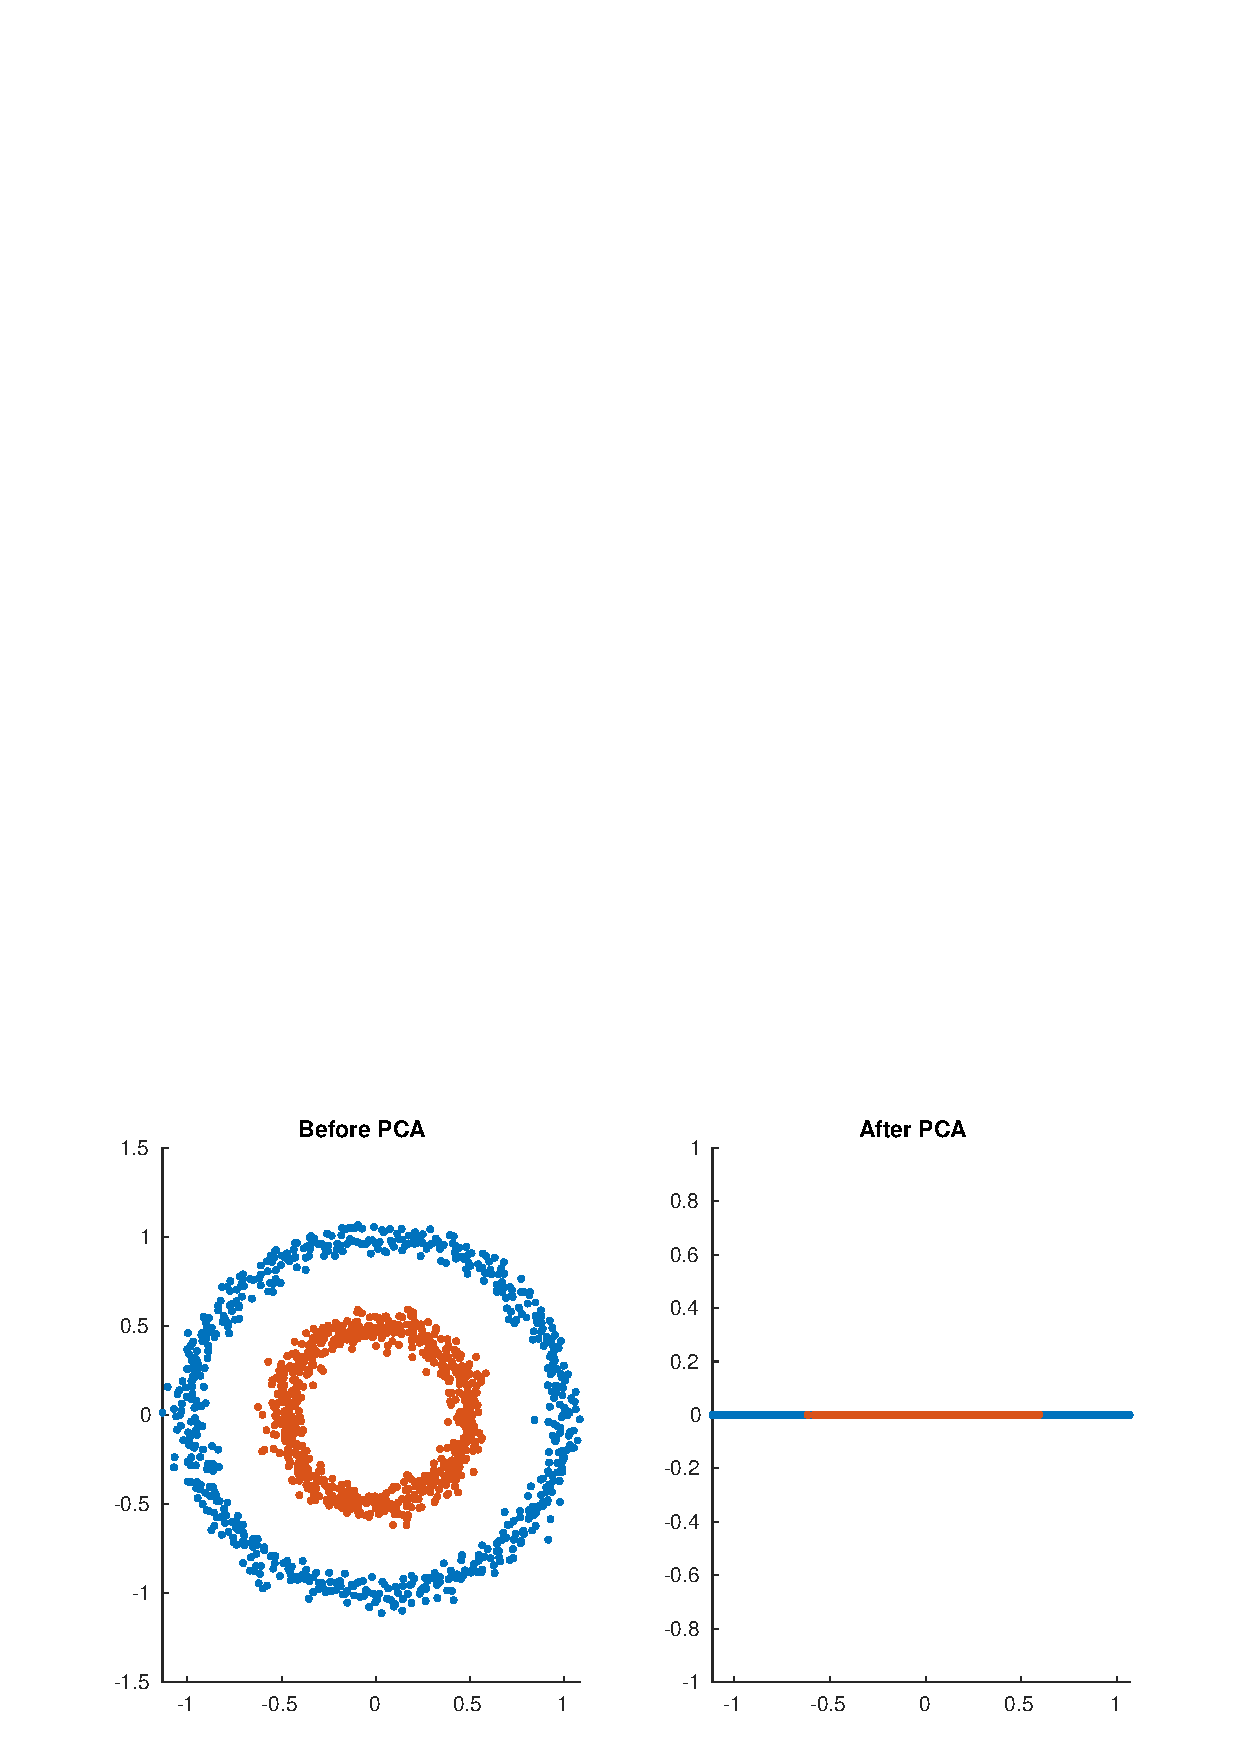
\includegraphics[width=\textwidth]{pic7.jpg}
			\end{figure}
			\item 
			مشکل۱: تفسیرناپذیری
		\begin{Large}
			\[\Phi(X)W\qquad\qquad\Phi(XW)\]
		\end{Large}
			\item 
			مشکل۲: عدم استفاده از برچسب داده‌ها در کاهش بُعد
		\end{itemize}
	\end{itemize}
\end{rawslide}
\begin{rawslide}
	\begin{itemize}
		\item \large\lr{IKDR}\normalsize
		\begin{itemize}
			\item 
			لزوم وجود یک معیار وابستگی
			\Large
			\[\max_W \;\;\mathrm{DEP}(XW,Y)\qquad \mathrm{s.t. } \;W^\top W = I\]
			\normalsize
			\item 
			معیار وابستگی
			\large\lr{HSIC}\normalsize
			
			\begin{equation*}
			\mathrm{MMD}(P, Q) = \norm{\mathbb{E}_{P}\left[ k(., X)\right] - \mathbb{E}_{Q}\left[ k(., X)\right]}_\mathcal{H}
			\end{equation*}
			\begin{equation*}
			\mathrm{HSIC}_k(X, Y) \triangleq \mathrm{MMD}_k(P_XP_Y, P_{XY})
			\end{equation*}
			\pause
			\item 
			تخمین 
			\large\lr{ HSIC}\normalsize
			از روی داده‌ها
			\begin{flalign*}
			\HSIC(XW, Y) &= \frac{1}{(n-1)^2} \tr (K_{XW}HK_YH)\\
			&= \frac{1}{(n-1)^2} \tr (HK_YHK_{XW})\\
			&= \frac{1}{(n-1)^2} \tr (\Gamma K_{XW})
			\end{flalign*}
		\end{itemize}
	\end{itemize}
\end{rawslide}
\begin{rawslide}
	\begin{itemize}
		\item 
		حلّ مسأله‌ی
		\large\lr{IKDR}\normalsize
		\begin{itemize}
			\item 
			یک مسأله‌ی بهینه‌سازی غیرمحدّب و به شدّت غیرخطّی
			\item 
			راه‌حل‌های قبلی موجود برای حلّ این مسأله
			\begin{itemize}
				\item \large\lr{Stiefel Manifold}\normalsize
				\item \large\lr{Grassman Manifold}\normalsize
				\item \large\lr{Dimension Growth}\normalsize
			\end{itemize}  
			\item 
			بهترین راه‌حل: الگوریتم 
			\large\lr{ Iterative Spectral Method (ISM)}\normalsize
			\begin{itemize}
				\item 
				پیاده‌سازی ساده‌تر
				\item 
				بسیار سریع‌تر از روش‌های قبلی
				\item 
				دچار مشکل‌ نشدن در نقاط زینی
				\item 
				تضمین تئوری فقط برای کرنل گاوسی
			\end{itemize}
		\item 
		هدف مقاله: تعمیم الگوریتم 
		\large\lr{ ISM}\normalsize
		به خانواده‌ی وسیع‌تری از کرنل‌ها
		\end{itemize}
	\end{itemize}
\end{rawslide}
\SecSlide[ISM]{\Huge\lr{Iterative Spectral Method}\normalsize}
\begin{rawslide}
	\subsection{ایده‌ی الگوریتم
	\large\lr{ ISM}\normalsize}		
		\begin{block}{تعریف کرنل‌
			\Large\lr{ ISM}\normalsize
		}
			\label{ISM-def}
			کرنل متقارن و مثبت معین
			$k(., .)$،
			یک کرنل 
			\lr{ISM}
			است، اگر دو بار مشتق‌پذیر باشد و برای آن داشته باشیم:
			\begin{equation}
			\forall \bx_i, \; \bx_j \in \R^d \;\;
			k(\bx_iW, \bx_jW) = f(\beta_{ij})
			\end{equation}
			که در آن
			\begin{equation}
			\beta_{ij} = a(\bx_i, \bx_j)^\top WW^\top b(\bx_i, \bx_j).
			\end{equation}
		\end{block}
	\begin{itemize}
		\item 
		مسأله‌ی بهینه‌سازی الگوریتم
		\large\lr{ IKDR}\normalsize:
		\[\max_W \;\; \tr(\Gamma K_{XW})\;\;\;\mathrm{s.t.}\;\;\;W^\top W=I\]
	\end{itemize}
\end{rawslide}
\begin{rawslide}
	مسأله‌ی بهینه‌سازی الگوریتم
	\large\lr{IKDR}\normalsize:\hfill
	$\max_W \;\; \tr(\Gamma K_{XW})\;\;\;\mathrm{s.t.}\;\;\;W^\top W=I$
	\begin{block}{قضیه}
		اگر
		\[-\frac{1}{2}\sum_{ij}{\Gamma_{ij} f'(\mathbf{a}^{T}WW^{T}\mathbf{b})} (\mathbf{b}\mathbf{a}^\top  + \mathbf{a}\mathbf{b}^\top )W - W \Lambda = 0.\]
		باشد، شرایط مرتبه‌ی اوّل مسأله‌ی بهینه‌سازی
		\large\lr{ IKDR}\normalsize
		برقرار می‌شود.
		این به آن معناست که 
		$W$
		باید شامل بردارهای ویژه‌ی ماتریس
		\[\Phi= -\frac{1}{2}\sum_{ij}{\Gamma_{ij} f'(\mathbf{a}^{T}WW^{T}\mathbf{b})} (\mathbf{b}\mathbf{a}^\top  + \mathbf{a}\mathbf{b}^\top )\]
		باشد. هم‌چنین اگر 
		$W$
		شامل بردارویژه‌های متناظر با کوچک‌ترین مقادیر ویژه‌ی 
		$\Phi$
		باشد، در شرایط مرتبه‌ی دوم مسأله‌ی بهینه‌سازی
		\large\lr{ IKDR}\normalsize
		هم صدق می‌کند.
		
	\end{block}
%		لاگرانژین مسأله:
%		\begin{align*}
%		\begin{split}
%		\mathcal{L}(W, \Lambda) = -\sum_{ij}
%		\Gamma_{ij} f(\mathbf{a}^{T}WW^{T}\mathbf{b}) 
%		- \tr[\Lambda(W^{T}W-I)]. \label{eq:Lagrangian}
%		\end{split}
%		\end{align*}
%		\item 
%		شرایط مرتبه‌ی اوّل:
%		\begin{flalign*}
%		\nabla_W \mathcal{L}(W, \Lambda) &= 
%		-\sum_{ij}{\Gamma_{ij} f'(\mathbf{a}^{T}WW^{T}\mathbf{b})} (\mathbf{b}\mathbf{a}^\top  + \mathbf{a}\mathbf{b}^\top )W - 2 W \Lambda= 0
%		\end{flalign*}
%		\begin{itemize}
%		\item 
%		تعریف می‌کنیم:
%		\[A = \mathbf{b}\mathbf{a}^\top  + \mathbf{a}\mathbf{b}^\top\]
%		\[\Psi_{i,j} = -\frac{1}{2}\Gamma_{i,j}f'(\mathbf{a}^{T}WW^{T}\mathbf{b})\]
%		\[\Phi = \sum_{i, j} \Psi_{ij}A_{i, j}\]
%		\item 
%		در نتیجه:
%		\[\Phi W = W \Lambda\]
%	\end{itemize}
\end{rawslide}
\begin{rawslide}
	\begin{itemize}
		\item 
		الگوریتم
		\large\lr{ISM}\normalsize:
		\begin{latin}
			\setstretch{1.5}
			\begin{algorithm}[H]
				\SetAlgoLined
				\KwIn{Data $X$, kernel, Subspace Dimension $q$}
				\KwOut{Projected subspace $W$} 
				\textbf{Initialization:} Initialize $\Phi_0$.
				
				Set $W_0$ to Dominant Eigenvectors of  of $\Phi_0$
				
				\While{ $||\Lambda_i - \Lambda_{i-1}||_2/||\Lambda_i||_2 < \delta$ }{
				
				Compute $\Phi$ with $W_{k-1}$
				
				Set $W_k$ to Dominant Eigenvectors of $\Phi$
			}
				
				\caption{ISM Algorithm}
				\label{alg:ism}
			\end{algorithm}   
		\end{latin}
		\normalsize
		\item 
		انتخاب یک شرط اوّلیّه‌ی مناسب:
		$\Phi_0$
	\end{itemize}
	\pause
	\begin{block}{قضیه}
		هر ترکیب خطّی با ضرایب مثبت ازکرنل‌های
		\large\lr{ISM}\normalsize،
		خود یک کرنل 
			\large\lr{ ISM}\normalsize
			است و ماتریس
			$\Phi$
			آن، از ترکیب خطّی ماتریس‌های
			$\Phi$
			کرنل‌های اوّلیه با همان ضرایب به دست می‌آید.
	\end{block}
\end{rawslide}
\SecSlide{کاربردها}
\begin{rawslide}
	\subsection{کاربردهای الگوریتم
	\Large\lr{ISM}\normalsize}
	\begin{itemize}
		\item 
		مسأله‌ی کاهش بُعد با نظارت
		\large\lr{(Supervised Dimension Reduction)}\normalsize
		\item 
		مسأله‌ی کاهش بُعد بدون نظارت
		\large\lr{(Unsupervised Dimension Reduction)}\normalsize
		\item 
		مسأله‌ی کاهش بُعد با نظارت ناقص
		\large\lr{(Semi-Supervised Dimension Reduction)}\normalsize
		\item 
		مسأله‌ی کاهش بعد جایگزین
		\large\lr{(Alternative Clustering)}
	\end{itemize}
\end{rawslide}
\SecSlide{شبیه‌سازی}
\begin{rawslide}
	
\end{rawslide}


\SecSlide{مراجع}
\begin{rawslide}
	\begin{tblock}
		\nocite{*}
		\bibliographystyle{unsrt-fa}
		\bibliography{Reference1}
	\end{tblock}
\end{rawslide}
\begin{comment}
\begin{rawslide}

\begin{thebibliography}{99}\vspace*{1.5cm}
\begin{tblock}
\begin{LTRbibitems}
\resetlatinfont
%مراجع لاتین👇

%\begin{flushleft}
\bibitem{MC}M. Crainic, R. Fernandes, Integrability of Lie brackets, \emph{Ann. of Math} \textbf{157} (2003) 575-620.

\bibitem{FB}Gh. Fasihi Ramandi, N. Boroojerdian, Forces Unification in The Framework of Transitive
Lie Algebroids,  \emph{Int.J.Theor.Phys} \textbf{54} (2015) 1581-1593.

\bibitem{CI}C. Ida, P. Popescu, On almost complex Lie algebroids, \emph{Mediterr. J. Math} (2015) 1-22.

\bibitem{RN} R. Nest, B. Tsygan, Deformations of symplectic Lie algebroids, deformations of holomorphic symplectic structures, and index theorems \emph{Asian J. Math.}, \textbf{5} (2001), 599–635.

%\end{flushleft}

\end{LTRbibitems}\end{tblock}
\end{thebibliography}\end{rawslide}
\end{comment}


\setcounter{bar}{\thepage}

\begin{comment}
\begin{titlepage}
\tikz[remember picture,overlay] \node[inner sep=0pt] at (current page.center) {\includegraphics[width=\paperwidth,height=\paperheight]{end}};
\end{titlepage}\setcounter{page}{\foo}
\end{comment}
%\begin{comment}
\begin{titlepage}
		\begin{tikzpicture}[remember picture,overlay]%
		\shade[color=red, top color=themeColor!15, bottom color=themeColor!80] (current page.north west) rectangle (current page.south east) node[pos=.5] {\color{mycolor1}{\Huge \rl{با تشکّر}}};
		\end{tikzpicture}%

	%\distance{0.1}
	%\centering
	%\vspace*{5cm}\hspace{-40mm}
	%\color{blue}{\Huge {با تشکّر}}
\end{titlepage}\setcounter{page}{\foo}
%\end{comment}
\end{document}